\section{Convergence Properties of CK}
We denote the $i$th realization of the knitted CNOT gate $N_{i}$ and the outcome of the $i$th realization of the quantum circuit projected onto the state $|\psi\rangle$ as $N_{i}^{|\psi\rangle}$, i.e., the outcome of the $5$th realization of the knitted quantum circuit projected onto the state $|01\rangle$ is $N_{5}^{|01\rangle}$.  
We initialize a qubit in the state 
\begin{equation}\label{eq:rand_init_state}
    |\psi\rangle = \begin{pmatrix}  -0.27274239+0.31439943 i\\-0.44805247+0.26438589i\\0.73699603+0.097286i\\-0.00941263+0.05828685i\end{pmatrix}, 
\end{equation}
and act on it with our knitted CNOT gate shown in figure~\ref{fig:knitted_circuit}.
The probabilities $p^{|\psi\rangle}$ of each outcome are
\begin{equation}
\begin{aligned}
    p^{|00>} =& 0.17323541288723698,\\
    p^{|01>} =& 0.0034859544864394004,\\
    p^{|10>} =& 0.5526277140317609,\\
    p^{|11>} =& 0.27065091470419295.
\end{aligned}
\end{equation}
We perform $10^{6}$ realizations of this knitted circuit and plot the cumulative results in figure~\ref{fig:cumulative_counts},
\begin{figure}[ht]
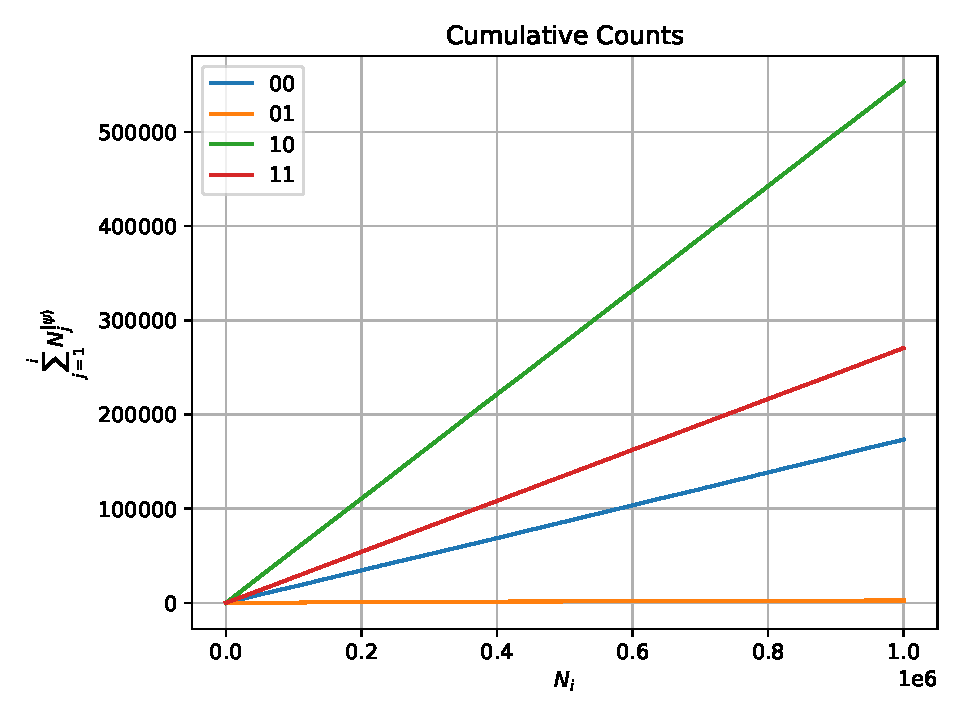
\includegraphics[width=0.48\textwidth]{figures/cumulative_counts.pdf}
\caption{
        The cumulative counts of each state for $N_{i}$ realizations of the knitted circuit of figure~\ref{fig:knitted_circuit} acting on the random initial state of eq.~\ref{eq:rand_init_state}.
}
\label{fig:cumulative_counts}
\end{figure}
the fraction of each outcome as a function of circuit realizations in figure~\ref{fig:raw_convergence},
\begin{figure}[ht]
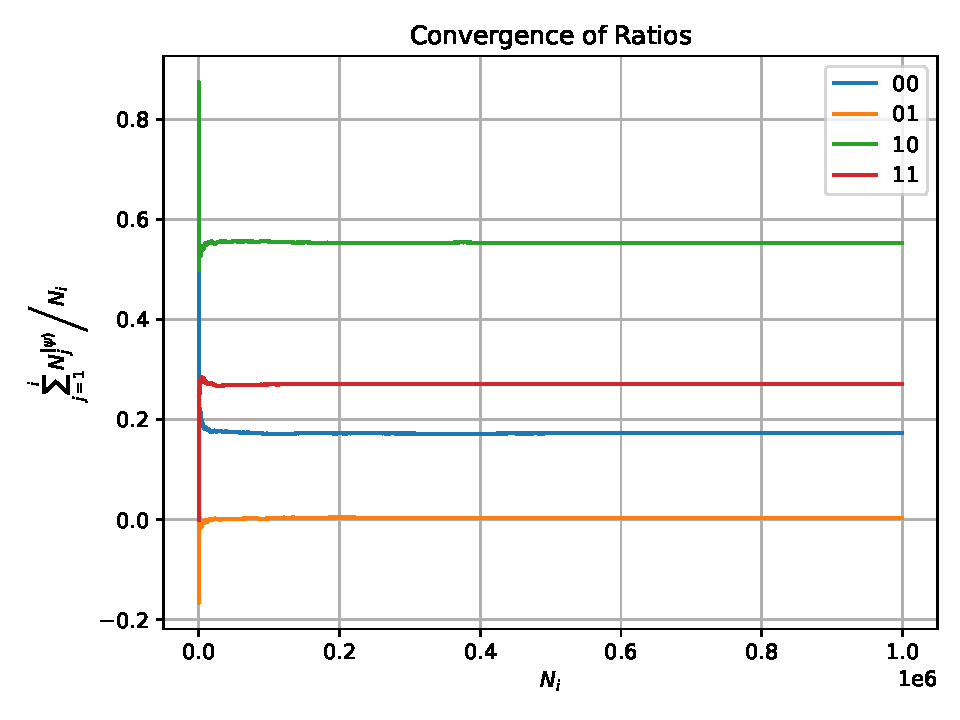
\includegraphics[width=0.48\textwidth]{figures/raw_convergence.pdf}
\caption{
        Figure~\ref{fig:cumulative_counts} divided by $N_{i}$, i.e., the ratio of cumulative counts of each state for $N_{i}$ realizations of the knitted circuit of figure~\ref{fig:knitted_circuit} to $N_{i}$; the initial state is given in eq.~\ref{eq:rand_init_state}.
}
\label{fig:raw_convergence}
\end{figure}
the difference between these fractions and the analytic expectations.
\begin{figure}[ht]
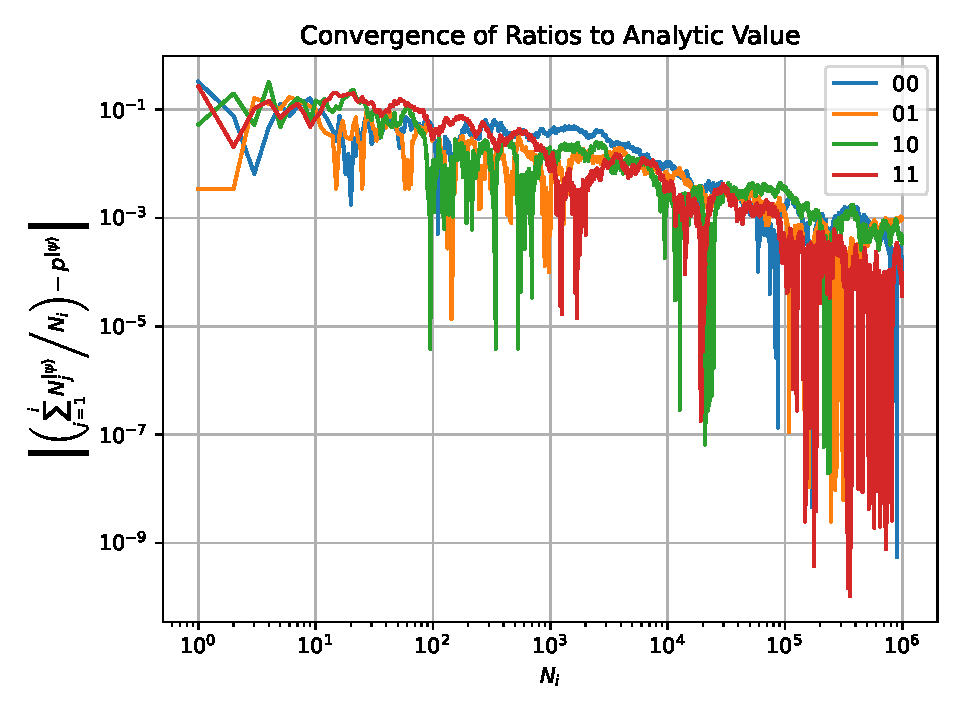
\includegraphics[width=0.48\textwidth]{figures/convergence.pdf}
\caption{
        The absolute value of the difference of figure~\ref{fig:raw_convergence} and the analytic analytic probabilities, i.e., the difference of the ratio of the cumulative counts of each state for $N_{i}$ realizations of the knitted circuit of figure~\ref{fig:knitted_circuit} to $N_{i}$ and the analytic probabilities; the initial state is given in eq.~\ref{eq:rand_init_state}.
}
\label{fig:convergence}
\end{figure}
As the ratio fluctuates above and below the analytic probability, the former quantity will display excursions to $0$ manifest in figure~\ref{fig:convergence} as deviations from the general $N^{-\frac{1}{2}}$ scaling.
To remedy this, we average each point in figure~\ref{fig:convergence} with all previous points; these results are displayed in figure~\ref{fig:smoothed_convergence}.
\begin{figure}[ht]
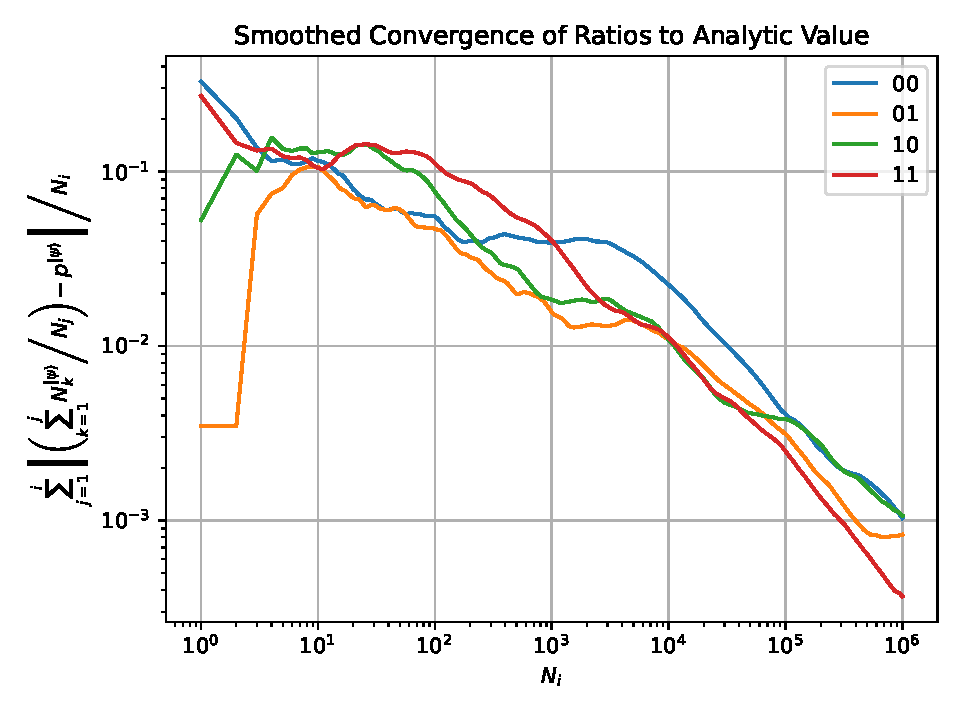
\includegraphics[width=0.48\textwidth]{figures/smoothed_convergence.pdf}
\caption{
        Each point of figure~\ref{fig:convergence} averaged with all preceeding points, i.e., the running average of the difference of the ratio of the cumulative counts of each state for $N_{i}$ realizations of the knitted circuit of figure~\ref{fig:knitted_circuit} to $N_{i}$ and the analytic probabilities; the initial state is given in eq.~\ref{eq:rand_init_state}.
}
\label{fig:smoothed_convergence}
\end{figure}

\begin{figure}[h]
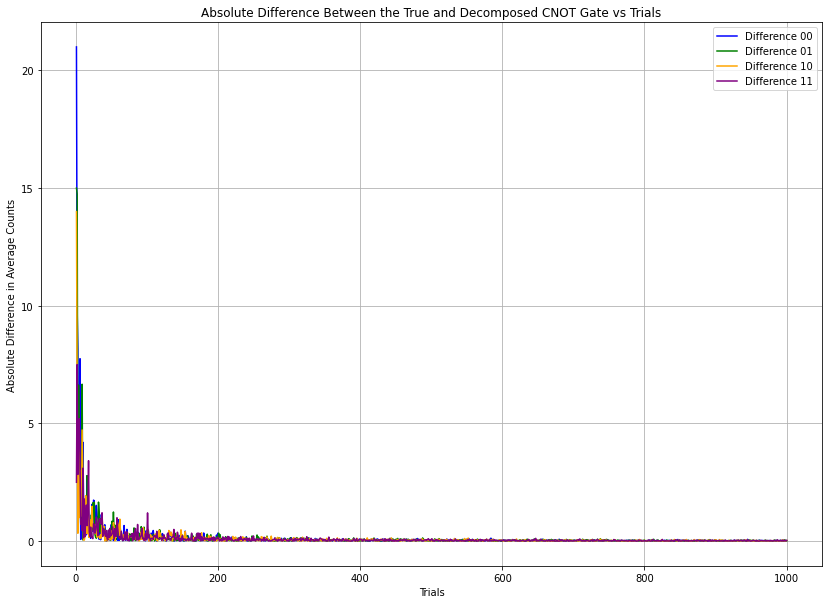
\includegraphics[width=0.5\textwidth]{figures/useable num - no error inc.png}
\caption{This figure displays the difference in average measured counts per state for the CNOT Decomposition and Qiskit's CNOT gate for a random initial state.}
\label{fig:figure2}
\end{figure}